\documentclass[12pt, a4paper]{article}
\usepackage{../notesheets}
%%%%%%%%%%%%%%%%%%%%%%%%%%%%%%%%%%%%%%%%%%%%%%%%%% 
\author{Math 1220}
\title{Notesheet. Section 8.7+8.8: Double Integrals + Geometric
  Applications Part 2}
\date{}

\begin{document}
\maketitle
\nameline
%%%%%%%%%%%%%%%%%%%%%%%%%%%%%%%%%%%%%%%%%%%%%%%%%%
\begin{ex}
  Evaluate \[
    \int_0^2 \int_{x^2}^4 e^{y^2}\ dy \dx
  \]
\end{ex}
\begin{thrm}
  If \(f(x,y)\) is integrable over the plane region \(R\), then its
  average value over \(R\) is given by \[
    \iint_R
  \]
\end{thrm}
\begin{ex}
  Find the average value of \(f(x,y) = 6x^2y\) over \(R = \{(x,y) \mid
  0 \leq x \leq 1; 0 \leq y \leq 3\}\). 
\end{ex}
\pagebreak
\begin{ex}
  Find the average value of \(f(x,y) = 6x^2 y\) over \(R\) bounded by
  \(y=1\), \(x=y\), and \(x=-y\).
\end{ex}
\begin{ex}
  Calculate the volume of the following solid:\\
  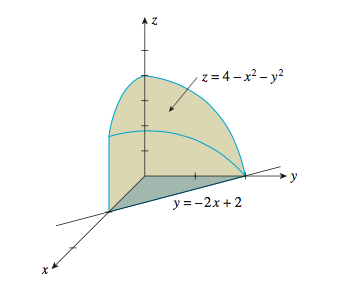
\includegraphics[scale=0.7]{images/solid-for-volume-calc}
\end{ex}
%%%%%%%%%%%%%%%%%%%%%%%%%%%%%%%%%%%%%%%%%%%%%%%%%% 
\end{document}
